Веб-приложение состоит из двух основных частей: back-end и front-end. Back-end -- это сам веб-сервер,
который осуществляет обработку запросов пользователей, получение и обработку данных.
Front-end -- это пользовательский интерфейс, визуализирующий полученные от back-end данные в понятный вид.
С помощью этого интерфейса пользователь способен не только получать, но и передавать данные на back-end.

Back-end составляющая сервиса реализована на языке Python 3, с использованием фреймворка Flask~---
обработка HTTP запросов пользователей, библиотеки Pandas~--- обработка и хранение данных, Scikit-learn~--- вычисление TF-IDF,
алгоритмы KMeans и линейный SVM, а также pymystem3 для лемматизации слов.

Структура приложения показана на рисунке \ref{server_struct}.
\begin{figure}[h]
    \centering
    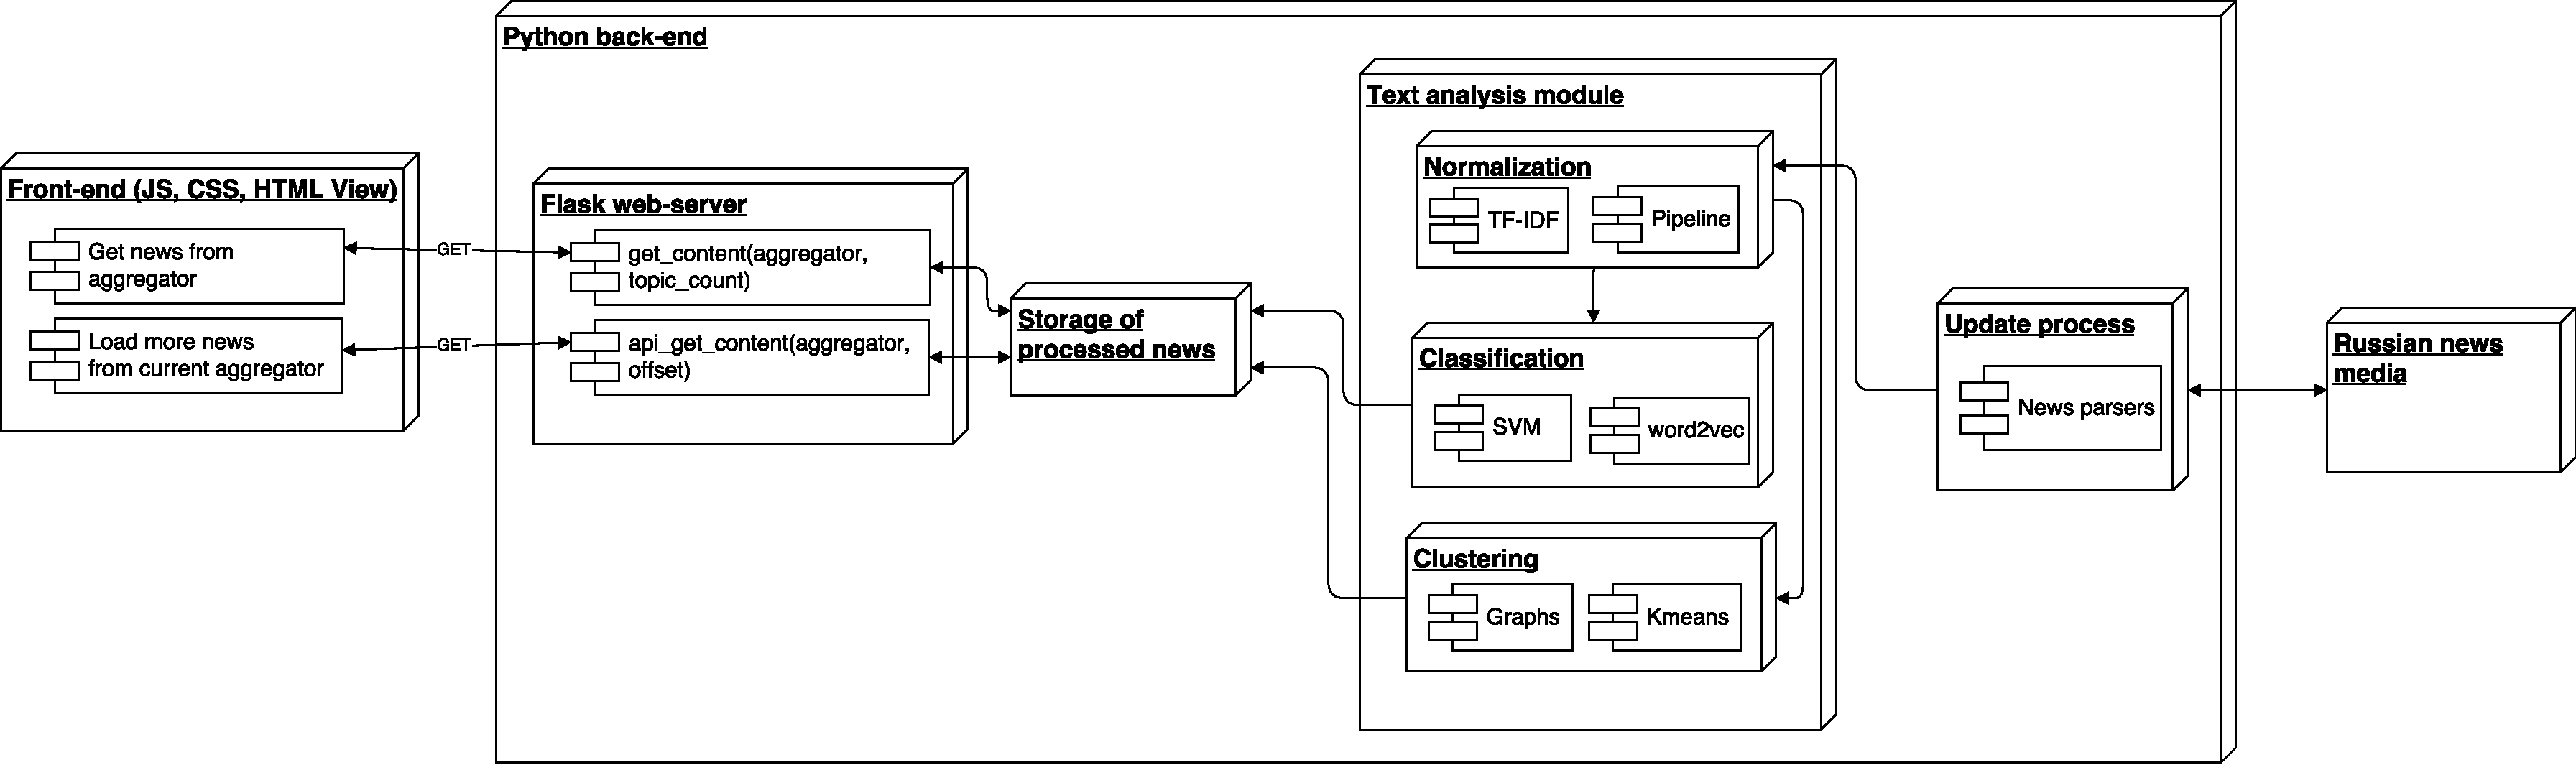
\includegraphics[width=1\textwidth]{server_infrastructure.pdf}
    \caption{Структура сервера}
    \label{server_struct}
\end{figure}

Back-end разделён на несколько модулей: Flask веб-сервер, модуль парсеров (англ. parser) новостей, которые
с помощью параллельных процессов извлекают данные из сайтов СМИ, а также модуль анализа данных.

При запуске сервера происходит получение и обработка новостей за последние 12 часов.
После чего запускается отдельный процесс, отвечающий за актуальность данных: каждую минуту он
проверяет наличие новых статей, и, если такие есть, получает и отправляет их на обработку. При запросе с Front-end,
сервер не обрабатывает данные с нуля, а обращается к уже обработанным, хранящимся в кэше, данным.

Основной частью сервера является класс \verb|Analizer|, обрабатывающий полученные
новостные статьи.

Данный класс, имеет следующие методы:
\begin{itemize}
    \item \verb|Конструктор|. Параметры: список новостных статей с мета-данными.

    В конструкторе класса производится загрузка сохранённых моделей, определяются параметры моделей кластеризации, вызываются
    функции \verb|_data_to_pandas|, \verb|_classify|, \verb|_classify|, \verb|_aggregate|, \verb|_form_output|.

    \item \verb|append_data|. Параметры: список новостных статей с мета-данными.

    Функция отвечает за добавление новых данных. Вызываются те же методы, что и
    в конструкторе. Дополнительно удаляются устаревшие данные.

    \item \verb|_data_to_pandas|. Параметры: список новостных статей с мета-данными. Возвращаемое значение: \verb|Pandas Dataframe|, в котором 
    хранится вся информация об актуальных новостях.

    Список новостей конвертируется в таблицу \verb|Pandas Dataframe|, из которой
    удаляются дубликаты, лишние мета-данные, происходит сортировка по дате 
    публикации статьи. Вызывается функция \verb|_norimalize|.

    \item \verb|_norimalize|. Параметры: \verb|Pandas Dataframe|.

    Происходит вызов конвеера функций нормализации текста. К таблице
    добавляются нормализованные текст и заголовок статей.

    \item \verb|_classify|. Параметры: \verb|Pandas Dataframe|.

    Вызываются функции классификации. Для каждого классификатора реализована отдельная функция, в которой к таблице добавляются колонка с тегами,
    полученными от данного классификатора.

    \item \verb|_aggregate|. Параметры: \verb|Pandas Dataframe| и 
    конфигурация алгоритмов кластеризации.

    Вызываются функции кластеризации: \verb|_aggregate_Kmeans|,
    \verb|_aggregate_graphs|.

    Для каждого алгоритма кластеризации реализована отдельная функция, которая возвращают список кластеров, каждый кластер представляет
    собой список ID --- индекс новости в таблице \verb|Pandas Dataframe|.

    \item \verb|_sort_groups|. Параметры: список кластеров, полученный от
    алгоритмов кластеризации. Возвращает отсортированный список кластеров.

    Фильтрует кластеры, в которых меньше двух новостей, после чего сортирует кластеры по среднему времени публикации.
    Затем происходит сортировка новостей внутри кластеров по времени их публикации.

    \item \verb|_get_avg_time|. Параметры: кластер. Возвращает среднее время
    в кластере.

    Преобразовывает даты публикации каждой новости кластера в Unix-timestamp и
    считает от них среднее.

    \item \verb|_get_TFIDF|. Параметры: \verb|Pandas Dataframe|.
    Возвращает модель TF-IDF и матрицу векторизованных новостей.

    \item \verb|_class_to_str|. Параметры: id класса.
    Возвращает название класса.

    \item \verb|_cut_text|. Параметры: текст.
    Возвращает первый абзац текста.

    \item \verb|_date_to_str|. Параметры: дата публикации.
    Возвращает дату в виде строки в заданном формате.

    \item \verb|_form_output|. Параметры: \verb|Pandas Dataframe|, список
    кластеров.

    Формирует данные в формате JSON и сохраняет их.

    \item \verb|get_data|. Параметров нет.
    Возвращает готовые данные в формате JSON и дату самой актуальной новости.

\end{itemize}
% \subsection{Back-end часть}
% \subsection{Front-end часть}